\section{Exercises}
    Reminder.
    \begin{figure}[H]
        \centering
        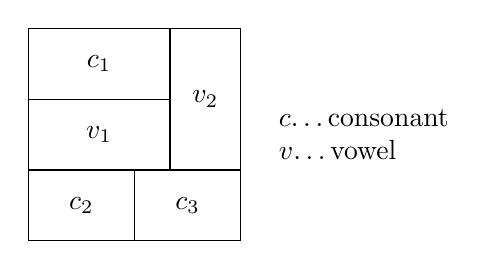
\begin{tikzpicture}[scale=0.9]
            \draw (0,2) rectangle (2,3) node[pos=.5] {$c_1$};
            \draw (0,1) rectangle (2,2) node[pos=.5] {$v_1$};
            \draw (2,1) rectangle (3,3) node[pos=.5] {$v_2$};
            \draw (0,0) rectangle (1.5,1) node[pos=.5] {$c_2$};
            \draw (1.5,0) rectangle (3,1) node[pos=.5] {$c_3$};
            \node[anchor=west, align=left] at (3.4,1.5) {$c$\ldots consonant\\ $v$\ldots vowel};
        \end{tikzpicture}
        \caption*{Reminder: Syllable Block}
    \end{figure}

    \begin{equation}
        \begin{pmatrix} \pmb{\text{\Large hangul letter}} \\ \boxed{\text{position in Block}} \\ \text{default sound} \\ \text{special case}\end{pmatrix}
    \end{equation}

    \begin{align}
        \textbf{\Huge } &= 
        \underbrace{
            \begin{pmatrix}\pmb{\text{\Large }}\\\boxed{\mathrm{c}_1}\\ \mathrm{}\\ \mathrm{} \end{pmatrix}
        }_{\mathrm{c}_i}
        +
        \underbrace{
            \begin{pmatrix}             
                \pmb{\text{\Large }}&\pmb{\text{\Large }}\\
                \boxed{\mathrm{v}_1}&\boxed{\mathrm{v}_2}\\
                \mathrm{}&\mathrm{}\\
                \mathrm{}&\mathrm{}
            \end{pmatrix}
        }_{\mathrm{v}_t}
        +
        \underbrace{
            \begin{pmatrix}
                \pmb{\text{\Large }} & \pmb{\text{\Large }}\\
                \boxed{\mathrm{c}_2} & \boxed{\mathrm{c}_3}\\
                \mathrm{} & \mathrm{}\\
                \mathrm{} & \mathrm{}
            \end{pmatrix}
        }_{\mathrm{c}_o}
        \\&=
        \begin{pmatrix}
            \pmb{\text{\Large }} & \pmb{\text{\Large }} & \pmb{\text{\Large }}\\
            \boxed{\mathrm{c}_i} & \boxed{\mathrm{v}_t} & \boxed{\mathrm{c}_o}\\
            \mathrm{} & \mathrm{} & \mathrm{}\\
            \mathrm{} & \mathrm{} & \mathrm{}
        \end{pmatrix}
        =
        \begin{pmatrix}\pmb{\text{\Large }}\\\boxed{\mathrm{syllable}}\\\mathrm{}\\\mathrm{}\end{pmatrix}_{\text{\footnotesize Answer:}}
    \end{align}
    
    \subsection{Initial consonant + single vowel}
    \begin{align}
        \textbf{\Huge 나} &= 
        \underbrace{
            \begin{pmatrix}\pmb{\text{\Large }}\\\boxed{\mathrm{c}_1}\\ \mathrm{}\\ \mathrm{} \end{pmatrix}
        }_{\mathrm{c}_i}
        +
        \underbrace{
            \begin{pmatrix}             
                \pmb{\text{\Large }}&\pmb{\text{\Large }}\\
                \boxed{\mathrm{v}_1}&\boxed{\mathrm{v}_2}\\
                \mathrm{}&\mathrm{}\\
                \mathrm{}&\mathrm{}
            \end{pmatrix}
        }_{\mathrm{v}_t}
        +
        \underbrace{
            \begin{pmatrix}
                \pmb{\text{\Large }} & \pmb{\text{\Large }}\\
                \boxed{\mathrm{c}_2} & \boxed{\mathrm{c}_3}\\
                \mathrm{} & \mathrm{}\\
                \mathrm{} & \mathrm{}
            \end{pmatrix}
        }_{\mathrm{c}_o}
        \\&=
        \begin{pmatrix}
            \pmb{\text{\Large }} & \pmb{\text{\Large }} & \pmb{\text{\Large }}\\
            \boxed{\mathrm{c}_i} & \boxed{\mathrm{v}_t} & \boxed{\mathrm{c}_o}\\
            \mathrm{} & \mathrm{} & \mathrm{}\\
            \mathrm{} & \mathrm{} & \mathrm{}
        \end{pmatrix}
        =
        \begin{pmatrix}\pmb{\text{\Large }}\\\boxed{\mathrm{syllable}}\\\mathrm{}\\\mathrm{}\end{pmatrix}_{\text{\footnotesize Answer: na}}
    \end{align}\\

    \begin{align}
        \textbf{\Huge 미} &= 
        \underbrace{
            \begin{pmatrix}\pmb{\text{\Large }}\\\boxed{\mathrm{c}_1}\\ \mathrm{}\\ \mathrm{} \end{pmatrix}
        }_{\mathrm{c}_i}
        +
        \underbrace{
            \begin{pmatrix}             
                \pmb{\text{\Large }}&\pmb{\text{\Large }}\\
                \boxed{\mathrm{v}_1}&\boxed{\mathrm{v}_2}\\
                \mathrm{}&\mathrm{}\\
                \mathrm{}&\mathrm{}
            \end{pmatrix}
        }_{\mathrm{v}_t}
        +
        \underbrace{
            \begin{pmatrix}
                \pmb{\text{\Large }} & \pmb{\text{\Large }}\\
                \boxed{\mathrm{c}_2} & \boxed{\mathrm{c}_3}\\
                \mathrm{} & \mathrm{}\\
                \mathrm{} & \mathrm{}
            \end{pmatrix}
        }_{\mathrm{c}_o}
        \\&=
        \begin{pmatrix}
            \pmb{\text{\Large }} & \pmb{\text{\Large }} & \pmb{\text{\Large }}\\
            \boxed{\mathrm{c}_i} & \boxed{\mathrm{v}_t} & \boxed{\mathrm{c}_o}\\
            \mathrm{} & \mathrm{} & \mathrm{}\\
            \mathrm{} & \mathrm{} & \mathrm{}
        \end{pmatrix}
        =
        \begin{pmatrix}\pmb{\text{\Large }}\\\boxed{\mathrm{syllable}}\\\mathrm{}\\\mathrm{}\end{pmatrix}_{\text{\footnotesize Answer: mi}}
    \end{align}\\

    \begin{align}
        \textbf{\Huge 개} &= 
        \underbrace{
            \begin{pmatrix}\pmb{\text{\Large }}\\\boxed{\mathrm{c}_1}\\ \mathrm{}\\ \mathrm{} \end{pmatrix}
        }_{\mathrm{c}_i}
        +
        \underbrace{
            \begin{pmatrix}             
                \pmb{\text{\Large }}&\pmb{\text{\Large }}\\
                \boxed{\mathrm{v}_1}&\boxed{\mathrm{v}_2}\\
                \mathrm{}&\mathrm{}\\
                \mathrm{}&\mathrm{}
            \end{pmatrix}
        }_{\mathrm{v}_t}
        +
        \underbrace{
            \begin{pmatrix}
                \pmb{\text{\Large }} & \pmb{\text{\Large }}\\
                \boxed{\mathrm{c}_2} & \boxed{\mathrm{c}_3}\\
                \mathrm{} & \mathrm{}\\
                \mathrm{} & \mathrm{}
            \end{pmatrix}
        }_{\mathrm{c}_o}
        \\&=
        \begin{pmatrix}
            \pmb{\text{\Large }} & \pmb{\text{\Large }} & \pmb{\text{\Large }}\\
            \boxed{\mathrm{c}_i} & \boxed{\mathrm{v}_t} & \boxed{\mathrm{c}_o}\\
            \mathrm{} & \mathrm{} & \mathrm{}\\
            \mathrm{} & \mathrm{} & \mathrm{}
        \end{pmatrix}
        =
        \begin{pmatrix}\pmb{\text{\Large }}\\\boxed{\mathrm{syllable}}\\\mathrm{}\\\mathrm{}\end{pmatrix}_{\text{\footnotesize Answer: gae}}
    \end{align}\\

    \begin{align}
        \textbf{\Huge 너} &= 
        \underbrace{
            \begin{pmatrix}\pmb{\text{\Large }}\\\boxed{\mathrm{c}_1}\\ \mathrm{}\\ \mathrm{} \end{pmatrix}
        }_{\mathrm{c}_i}
        +
        \underbrace{
            \begin{pmatrix}             
                \pmb{\text{\Large }}&\pmb{\text{\Large }}\\
                \boxed{\mathrm{v}_1}&\boxed{\mathrm{v}_2}\\
                \mathrm{}&\mathrm{}\\
                \mathrm{}&\mathrm{}
            \end{pmatrix}
        }_{\mathrm{v}_t}
        +
        \underbrace{
            \begin{pmatrix}
                \pmb{\text{\Large }} & \pmb{\text{\Large }}\\
                \boxed{\mathrm{c}_2} & \boxed{\mathrm{c}_3}\\
                \mathrm{} & \mathrm{}\\
                \mathrm{} & \mathrm{}
            \end{pmatrix}
        }_{\mathrm{c}_o}
        \\&=
        \begin{pmatrix}
            \pmb{\text{\Large }} & \pmb{\text{\Large }} & \pmb{\text{\Large }}\\
            \boxed{\mathrm{c}_i} & \boxed{\mathrm{v}_t} & \boxed{\mathrm{c}_o}\\
            \mathrm{} & \mathrm{} & \mathrm{}\\
            \mathrm{} & \mathrm{} & \mathrm{}
        \end{pmatrix}
        =
        \begin{pmatrix}\pmb{\text{\Large }}\\\boxed{\mathrm{syllable}}\\\mathrm{}\\\mathrm{}\end{pmatrix}_{\text{\footnotesize Answer: nuh}}
    \end{align}\\

    \begin{align}
        \textbf{\Huge 도} &= 
        \underbrace{
            \begin{pmatrix}\pmb{\text{\Large }}\\\boxed{\mathrm{c}_1}\\ \mathrm{}\\ \mathrm{} \end{pmatrix}
        }_{\mathrm{c}_i}
        +
        \underbrace{
            \begin{pmatrix}             
                \pmb{\text{\Large }}&\pmb{\text{\Large }}\\
                \boxed{\mathrm{v}_1}&\boxed{\mathrm{v}_2}\\
                \mathrm{}&\mathrm{}\\
                \mathrm{}&\mathrm{}
            \end{pmatrix}
        }_{\mathrm{v}_t}
        +
        \underbrace{
            \begin{pmatrix}
                \pmb{\text{\Large }} & \pmb{\text{\Large }}\\
                \boxed{\mathrm{c}_2} & \boxed{\mathrm{c}_3}\\
                \mathrm{} & \mathrm{}\\
                \mathrm{} & \mathrm{}
            \end{pmatrix}
        }_{\mathrm{c}_o}
        \\&=
        \begin{pmatrix}
            \pmb{\text{\Large }} & \pmb{\text{\Large }} & \pmb{\text{\Large }}\\
            \boxed{\mathrm{c}_i} & \boxed{\mathrm{v}_t} & \boxed{\mathrm{c}_o}\\
            \mathrm{} & \mathrm{} & \mathrm{}\\
            \mathrm{} & \mathrm{} & \mathrm{}
        \end{pmatrix}
        =
        \begin{pmatrix}\pmb{\text{\Large }}\\\boxed{\mathrm{syllable}}\\\mathrm{}\\\mathrm{}\end{pmatrix}_{\text{\footnotesize Answer: do}}
    \end{align}\\

    \begin{align}
        \textbf{\Huge 그} &= 
        \underbrace{
            \begin{pmatrix}\pmb{\text{\Large }}\\\boxed{\mathrm{c}_1}\\ \mathrm{}\\ \mathrm{} \end{pmatrix}
        }_{\mathrm{c}_i}
        +
        \underbrace{
            \begin{pmatrix}             
                \pmb{\text{\Large }}&\pmb{\text{\Large }}\\
                \boxed{\mathrm{v}_1}&\boxed{\mathrm{v}_2}\\
                \mathrm{}&\mathrm{}\\
                \mathrm{}&\mathrm{}
            \end{pmatrix}
        }_{\mathrm{v}_t}
        +
        \underbrace{
            \begin{pmatrix}
                \pmb{\text{\Large }} & \pmb{\text{\Large }}\\
                \boxed{\mathrm{c}_2} & \boxed{\mathrm{c}_3}\\
                \mathrm{} & \mathrm{}\\
                \mathrm{} & \mathrm{}
            \end{pmatrix}
        }_{\mathrm{c}_o}
        \\&=
        \begin{pmatrix}
            \pmb{\text{\Large }} & \pmb{\text{\Large }} & \pmb{\text{\Large }}\\
            \boxed{\mathrm{c}_i} & \boxed{\mathrm{v}_t} & \boxed{\mathrm{c}_o}\\
            \mathrm{} & \mathrm{} & \mathrm{}\\
            \mathrm{} & \mathrm{} & \mathrm{}
        \end{pmatrix}
        =
        \begin{pmatrix}\pmb{\text{\Large }}\\\boxed{\mathrm{syllable}}\\\mathrm{}\\\mathrm{}\end{pmatrix}_{\text{\footnotesize Answer: geww}}
    \end{align}\\

    \begin{align}
        \textbf{\Huge 효} &= 
        \underbrace{
            \begin{pmatrix}\pmb{\text{\Large }}\\\boxed{\mathrm{c}_1}\\ \mathrm{}\\ \mathrm{} \end{pmatrix}
        }_{\mathrm{c}_i}
        +
        \underbrace{
            \begin{pmatrix}             
                \pmb{\text{\Large }}&\pmb{\text{\Large }}\\
                \boxed{\mathrm{v}_1}&\boxed{\mathrm{v}_2}\\
                \mathrm{}&\mathrm{}\\
                \mathrm{}&\mathrm{}
            \end{pmatrix}
        }_{\mathrm{v}_t}
        +
        \underbrace{
            \begin{pmatrix}
                \pmb{\text{\Large }} & \pmb{\text{\Large }}\\
                \boxed{\mathrm{c}_2} & \boxed{\mathrm{c}_3}\\
                \mathrm{} & \mathrm{}\\
                \mathrm{} & \mathrm{}
            \end{pmatrix}
        }_{\mathrm{c}_o}
        \\&=
        \begin{pmatrix}
            \pmb{\text{\Large }} & \pmb{\text{\Large }} & \pmb{\text{\Large }}\\
            \boxed{\mathrm{c}_i} & \boxed{\mathrm{v}_t} & \boxed{\mathrm{c}_o}\\
            \mathrm{} & \mathrm{} & \mathrm{}\\
            \mathrm{} & \mathrm{} & \mathrm{}
        \end{pmatrix}
        =
        \begin{pmatrix}\pmb{\text{\Large }}\\\boxed{\mathrm{syllable}}\\\mathrm{}\\\mathrm{}\end{pmatrix}_{\text{\footnotesize Answer: hyo}}
    \end{align}
    \subsection{Initial consonant + compound vowel}
    \begin{align}
        \textbf{\Huge 왜} &= 
        \underbrace{
            \begin{pmatrix}\pmb{\text{\Large }}\\\boxed{\mathrm{c}_1}\\ \mathrm{}\\ \mathrm{} \end{pmatrix}
        }_{\mathrm{c}_i}
        +
        \underbrace{
            \begin{pmatrix}             
                \pmb{\text{\Large }}&\pmb{\text{\Large }}\\
                \boxed{\mathrm{v}_1}&\boxed{\mathrm{v}_2}\\
                \mathrm{}&\mathrm{}\\
                \mathrm{}&\mathrm{}
            \end{pmatrix}
        }_{\mathrm{v}_t}
        +
        \underbrace{
            \begin{pmatrix}
                \pmb{\text{\Large }} & \pmb{\text{\Large }}\\
                \boxed{\mathrm{c}_2} & \boxed{\mathrm{c}_3}\\
                \mathrm{} & \mathrm{}\\
                \mathrm{} & \mathrm{}
            \end{pmatrix}
        }_{\mathrm{c}_o}
        \\&=
        \begin{pmatrix}
            \pmb{\text{\Large }} & \pmb{\text{\Large }} & \pmb{\text{\Large }}\\
            \boxed{\mathrm{c}_i} & \boxed{\mathrm{v}_t} & \boxed{\mathrm{c}_o}\\
            \mathrm{} & \mathrm{} & \mathrm{}\\
            \mathrm{} & \mathrm{} & \mathrm{}
        \end{pmatrix}
        =
        \begin{pmatrix}\pmb{\text{\Large }}\\\boxed{\mathrm{syllable}}\\\mathrm{}\\\mathrm{}\end{pmatrix}_{\text{\footnotesize Answer: wae}}
    \end{align}\\

    \begin{align}
        \textbf{\Huge 위} &= 
        \underbrace{
            \begin{pmatrix}\pmb{\text{\Large }}\\\boxed{\mathrm{c}_1}\\ \mathrm{}\\ \mathrm{} \end{pmatrix}
        }_{\mathrm{c}_i}
        +
        \underbrace{
            \begin{pmatrix}             
                \pmb{\text{\Large }}&\pmb{\text{\Large }}\\
                \boxed{\mathrm{v}_1}&\boxed{\mathrm{v}_2}\\
                \mathrm{}&\mathrm{}\\
                \mathrm{}&\mathrm{}
            \end{pmatrix}
        }_{\mathrm{v}_t}
        +
        \underbrace{
            \begin{pmatrix}
                \pmb{\text{\Large }} & \pmb{\text{\Large }}\\
                \boxed{\mathrm{c}_2} & \boxed{\mathrm{c}_3}\\
                \mathrm{} & \mathrm{}\\
                \mathrm{} & \mathrm{}
            \end{pmatrix}
        }_{\mathrm{c}_o}
        \\&=
        \begin{pmatrix}
            \pmb{\text{\Large }} & \pmb{\text{\Large }} & \pmb{\text{\Large }}\\
            \boxed{\mathrm{c}_i} & \boxed{\mathrm{v}_t} & \boxed{\mathrm{c}_o}\\
            \mathrm{} & \mathrm{} & \mathrm{}\\
            \mathrm{} & \mathrm{} & \mathrm{}
        \end{pmatrix}
        =
        \begin{pmatrix}\pmb{\text{\Large }}\\\boxed{\mathrm{syllable}}\\\mathrm{}\\\mathrm{}\end{pmatrix}_{\text{\footnotesize Answer: wi}}
    \end{align}\\

    \begin{align}
        \textbf{\Huge 뭐} &= 
        \underbrace{
            \begin{pmatrix}\pmb{\text{\Large }}\\\boxed{\mathrm{c}_1}\\ \mathrm{}\\ \mathrm{} \end{pmatrix}
        }_{\mathrm{c}_i}
        +
        \underbrace{
            \begin{pmatrix}             
                \pmb{\text{\Large }}&\pmb{\text{\Large }}\\
                \boxed{\mathrm{v}_1}&\boxed{\mathrm{v}_2}\\
                \mathrm{}&\mathrm{}\\
                \mathrm{}&\mathrm{}
            \end{pmatrix}
        }_{\mathrm{v}_t}
        +
        \underbrace{
            \begin{pmatrix}
                \pmb{\text{\Large }} & \pmb{\text{\Large }}\\
                \boxed{\mathrm{c}_2} & \boxed{\mathrm{c}_3}\\
                \mathrm{} & \mathrm{}\\
                \mathrm{} & \mathrm{}
            \end{pmatrix}
        }_{\mathrm{c}_o}
        \\&=
        \begin{pmatrix}
            \pmb{\text{\Large }} & \pmb{\text{\Large }} & \pmb{\text{\Large }}\\
            \boxed{\mathrm{c}_i} & \boxed{\mathrm{v}_t} & \boxed{\mathrm{c}_o}\\
            \mathrm{} & \mathrm{} & \mathrm{}\\
            \mathrm{} & \mathrm{} & \mathrm{}
        \end{pmatrix}
        =
        \begin{pmatrix}\pmb{\text{\Large }}\\\boxed{\mathrm{syllable}}\\\mathrm{}\\\mathrm{}\end{pmatrix}_{\text{\footnotesize Answer: mwo}}
    \end{align}\\

    \begin{align}
        \textbf{\Huge 의} &= 
        \underbrace{
            \begin{pmatrix}\pmb{\text{\Large }}\\\boxed{\mathrm{c}_1}\\ \mathrm{}\\ \mathrm{} \end{pmatrix}
        }_{\mathrm{c}_i}
        +
        \underbrace{
            \begin{pmatrix}             
                \pmb{\text{\Large }}&\pmb{\text{\Large }}\\
                \boxed{\mathrm{v}_1}&\boxed{\mathrm{v}_2}\\
                \mathrm{}&\mathrm{}\\
                \mathrm{}&\mathrm{}
            \end{pmatrix}
        }_{\mathrm{v}_t}
        +
        \underbrace{
            \begin{pmatrix}
                \pmb{\text{\Large }} & \pmb{\text{\Large }}\\
                \boxed{\mathrm{c}_2} & \boxed{\mathrm{c}_3}\\
                \mathrm{} & \mathrm{}\\
                \mathrm{} & \mathrm{}
            \end{pmatrix}
        }_{\mathrm{c}_o}
        \\&=
        \begin{pmatrix}
            \pmb{\text{\Large }} & \pmb{\text{\Large }} & \pmb{\text{\Large }}\\
            \boxed{\mathrm{c}_i} & \boxed{\mathrm{v}_t} & \boxed{\mathrm{c}_o}\\
            \mathrm{} & \mathrm{} & \mathrm{}\\
            \mathrm{} & \mathrm{} & \mathrm{}
        \end{pmatrix}
        =
        \begin{pmatrix}\pmb{\text{\Large }}\\\boxed{\mathrm{syllable}}\\\mathrm{}\\\mathrm{}\end{pmatrix}_{\text{\footnotesize Answer: ui}}
    \end{align}
    \subsection{Initial consonant + single vowel + optional consonant}
    \begin{align}
        \textbf{\Huge 산} &= 
        \underbrace{
            \begin{pmatrix}\pmb{\text{\Large }}\\\boxed{\mathrm{c}_1}\\ \mathrm{}\\ \mathrm{} \end{pmatrix}
        }_{\mathrm{c}_i}
        +
        \underbrace{
            \begin{pmatrix}             
                \pmb{\text{\Large }}&\pmb{\text{\Large }}\\
                \boxed{\mathrm{v}_1}&\boxed{\mathrm{v}_2}\\
                \mathrm{}&\mathrm{}\\
                \mathrm{}&\mathrm{}
            \end{pmatrix}
        }_{\mathrm{v}_t}
        +
        \underbrace{
            \begin{pmatrix}
                \pmb{\text{\Large }} & \pmb{\text{\Large }}\\
                \boxed{\mathrm{c}_2} & \boxed{\mathrm{c}_3}\\
                \mathrm{} & \mathrm{}\\
                \mathrm{} & \mathrm{}
            \end{pmatrix}
        }_{\mathrm{c}_o}
        \\&=
        \begin{pmatrix}
            \pmb{\text{\Large }} & \pmb{\text{\Large }} & \pmb{\text{\Large }}\\
            \boxed{\mathrm{c}_i} & \boxed{\mathrm{v}_t} & \boxed{\mathrm{c}_o}\\
            \mathrm{} & \mathrm{} & \mathrm{}\\
            \mathrm{} & \mathrm{} & \mathrm{}
        \end{pmatrix}
        =
        \begin{pmatrix}\pmb{\text{\Large }}\\\boxed{\mathrm{syllable}}\\\mathrm{}\\\mathrm{}\end{pmatrix}_{\text{\footnotesize Answer: san}}
    \end{align}\\

    \begin{align}
        \textbf{\Huge 물} &= 
        \underbrace{
            \begin{pmatrix}\pmb{\text{\Large }}\\\boxed{\mathrm{c}_1}\\ \mathrm{}\\ \mathrm{} \end{pmatrix}
        }_{\mathrm{c}_i}
        +
        \underbrace{
            \begin{pmatrix}             
                \pmb{\text{\Large }}&\pmb{\text{\Large }}\\
                \boxed{\mathrm{v}_1}&\boxed{\mathrm{v}_2}\\
                \mathrm{}&\mathrm{}\\
                \mathrm{}&\mathrm{}
            \end{pmatrix}
        }_{\mathrm{v}_t}
        +
        \underbrace{
            \begin{pmatrix}
                \pmb{\text{\Large }} & \pmb{\text{\Large }}\\
                \boxed{\mathrm{c}_2} & \boxed{\mathrm{c}_3}\\
                \mathrm{} & \mathrm{}\\
                \mathrm{} & \mathrm{}
            \end{pmatrix}
        }_{\mathrm{c}_o}
        \\&=
        \begin{pmatrix}
            \pmb{\text{\Large }} & \pmb{\text{\Large }} & \pmb{\text{\Large }}\\
            \boxed{\mathrm{c}_i} & \boxed{\mathrm{v}_t} & \boxed{\mathrm{c}_o}\\
            \mathrm{} & \mathrm{} & \mathrm{}\\
            \mathrm{} & \mathrm{} & \mathrm{}
        \end{pmatrix}
        =
        \begin{pmatrix}\pmb{\text{\Large }}\\\boxed{\mathrm{syllable}}\\\mathrm{}\\\mathrm{}\end{pmatrix}_{\text{\footnotesize Answer: mool}}
    \end{align}\\

    \begin{align}
        \textbf{\Huge 강} &= 
        \underbrace{
            \begin{pmatrix}\pmb{\text{\Large }}\\\boxed{\mathrm{c}_1}\\ \mathrm{}\\ \mathrm{} \end{pmatrix}
        }_{\mathrm{c}_i}
        +
        \underbrace{
            \begin{pmatrix}             
                \pmb{\text{\Large }}&\pmb{\text{\Large }}\\
                \boxed{\mathrm{v}_1}&\boxed{\mathrm{v}_2}\\
                \mathrm{}&\mathrm{}\\
                \mathrm{}&\mathrm{}
            \end{pmatrix}
        }_{\mathrm{v}_t}
        +
        \underbrace{
            \begin{pmatrix}
                \pmb{\text{\Large }} & \pmb{\text{\Large }}\\
                \boxed{\mathrm{c}_2} & \boxed{\mathrm{c}_3}\\
                \mathrm{} & \mathrm{}\\
                \mathrm{} & \mathrm{}
            \end{pmatrix}
        }_{\mathrm{c}_o}
        \\&=
        \begin{pmatrix}
            \pmb{\text{\Large }} & \pmb{\text{\Large }} & \pmb{\text{\Large }}\\
            \boxed{\mathrm{c}_i} & \boxed{\mathrm{v}_t} & \boxed{\mathrm{c}_o}\\
            \mathrm{} & \mathrm{} & \mathrm{}\\
            \mathrm{} & \mathrm{} & \mathrm{}
        \end{pmatrix}
        =
        \begin{pmatrix}\pmb{\text{\Large }}\\\boxed{\mathrm{syllable}}\\\mathrm{}\\\mathrm{}\end{pmatrix}_{\text{\footnotesize Answer: gang}}
    \end{align}\\

    \begin{align}
        \textbf{\Huge 옷} &= 
        \underbrace{
            \begin{pmatrix}\pmb{\text{\Large }}\\\boxed{\mathrm{c}_1}\\ \mathrm{}\\ \mathrm{} \end{pmatrix}
        }_{\mathrm{c}_i}
        +
        \underbrace{
            \begin{pmatrix}             
                \pmb{\text{\Large }}&\pmb{\text{\Large }}\\
                \boxed{\mathrm{v}_1}&\boxed{\mathrm{v}_2}\\
                \mathrm{}&\mathrm{}\\
                \mathrm{}&\mathrm{}
            \end{pmatrix}
        }_{\mathrm{v}_t}
        +
        \underbrace{
            \begin{pmatrix}
                \pmb{\text{\Large }} & \pmb{\text{\Large }}\\
                \boxed{\mathrm{c}_2} & \boxed{\mathrm{c}_3}\\
                \mathrm{} & \mathrm{}\\
                \mathrm{} & \mathrm{}
            \end{pmatrix}
        }_{\mathrm{c}_o}
        \\&=
        \begin{pmatrix}
            \pmb{\text{\Large }} & \pmb{\text{\Large }} & \pmb{\text{\Large }}\\
            \boxed{\mathrm{c}_i} & \boxed{\mathrm{v}_t} & \boxed{\mathrm{c}_o}\\
            \mathrm{} & \mathrm{} & \mathrm{}\\
            \mathrm{} & \mathrm{} & \mathrm{}
        \end{pmatrix}
        =
        \begin{pmatrix}\pmb{\text{\Large }}\\\boxed{\mathrm{syllable}}\\\mathrm{}\\\mathrm{}\end{pmatrix}_{\text{\footnotesize Answer: od}}
    \end{align}\\

    \begin{align}
        \textbf{\Huge 낮} &= 
        \underbrace{
            \begin{pmatrix}\pmb{\text{\Large }}\\\boxed{\mathrm{c}_1}\\ \mathrm{}\\ \mathrm{} \end{pmatrix}
        }_{\mathrm{c}_i}
        +
        \underbrace{
            \begin{pmatrix}             
                \pmb{\text{\Large }}&\pmb{\text{\Large }}\\
                \boxed{\mathrm{v}_1}&\boxed{\mathrm{v}_2}\\
                \mathrm{}&\mathrm{}\\
                \mathrm{}&\mathrm{}
            \end{pmatrix}
        }_{\mathrm{v}_t}
        +
        \underbrace{
            \begin{pmatrix}
                \pmb{\text{\Large }} & \pmb{\text{\Large }}\\
                \boxed{\mathrm{c}_2} & \boxed{\mathrm{c}_3}\\
                \mathrm{} & \mathrm{}\\
                \mathrm{} & \mathrm{}
            \end{pmatrix}
        }_{\mathrm{c}_o}
        \\&=
        \begin{pmatrix}
            \pmb{\text{\Large }} & \pmb{\text{\Large }} & \pmb{\text{\Large }}\\
            \boxed{\mathrm{c}_i} & \boxed{\mathrm{v}_t} & \boxed{\mathrm{c}_o}\\
            \mathrm{} & \mathrm{} & \mathrm{}\\
            \mathrm{} & \mathrm{} & \mathrm{}
        \end{pmatrix}
        =
        \begin{pmatrix}\pmb{\text{\Large }}\\\boxed{\mathrm{syllable}}\\\mathrm{}\\\mathrm{}\end{pmatrix}_{\text{\footnotesize Answer: nad}}
    \end{align}
    
    \subsection{Initial consonant + compound vowel + optional consonant}
    \begin{align}
        \textbf{\Huge 원} &= 
        \underbrace{
            \begin{pmatrix}\pmb{\text{\Large }}\\\boxed{\mathrm{c}_1}\\ \mathrm{}\\ \mathrm{} \end{pmatrix}
        }_{\mathrm{c}_i}
        +
        \underbrace{
            \begin{pmatrix}             
                \pmb{\text{\Large }}&\pmb{\text{\Large }}\\
                \boxed{\mathrm{v}_1}&\boxed{\mathrm{v}_2}\\
                \mathrm{}&\mathrm{}\\
                \mathrm{}&\mathrm{}
            \end{pmatrix}
        }_{\mathrm{v}_t}
        +
        \underbrace{
            \begin{pmatrix}
                \pmb{\text{\Large }} & \pmb{\text{\Large }}\\
                \boxed{\mathrm{c}_2} & \boxed{\mathrm{c}_3}\\
                \mathrm{} & \mathrm{}\\
                \mathrm{} & \mathrm{}
            \end{pmatrix}
        }_{\mathrm{c}_o}
        \\&=
        \begin{pmatrix}
            \pmb{\text{\Large }} & \pmb{\text{\Large }} & \pmb{\text{\Large }}\\
            \boxed{\mathrm{c}_i} & \boxed{\mathrm{v}_t} & \boxed{\mathrm{c}_o}\\
            \mathrm{} & \mathrm{} & \mathrm{}\\
            \mathrm{} & \mathrm{} & \mathrm{}
        \end{pmatrix}
        =
        \begin{pmatrix}\pmb{\text{\Large }}\\\boxed{\mathrm{syllable}}\\\mathrm{}\\\mathrm{}\end{pmatrix}_{\text{\footnotesize Answer: won}}
    \end{align}\\

    \begin{align}
        \textbf{\Huge 괜} &= 
        \underbrace{
            \begin{pmatrix}\pmb{\text{\Large }}\\\boxed{\mathrm{c}_1}\\ \mathrm{}\\ \mathrm{} \end{pmatrix}
        }_{\mathrm{c}_i}
        +
        \underbrace{
            \begin{pmatrix}             
                \pmb{\text{\Large }}&\pmb{\text{\Large }}\\
                \boxed{\mathrm{v}_1}&\boxed{\mathrm{v}_2}\\
                \mathrm{}&\mathrm{}\\
                \mathrm{}&\mathrm{}
            \end{pmatrix}
        }_{\mathrm{v}_t}
        +
        \underbrace{
            \begin{pmatrix}
                \pmb{\text{\Large }} & \pmb{\text{\Large }}\\
                \boxed{\mathrm{c}_2} & \boxed{\mathrm{c}_3}\\
                \mathrm{} & \mathrm{}\\
                \mathrm{} & \mathrm{}
            \end{pmatrix}
        }_{\mathrm{c}_o}
        \\&=
        \begin{pmatrix}
            \pmb{\text{\Large }} & \pmb{\text{\Large }} & \pmb{\text{\Large }}\\
            \boxed{\mathrm{c}_i} & \boxed{\mathrm{v}_t} & \boxed{\mathrm{c}_o}\\
            \mathrm{} & \mathrm{} & \mathrm{}\\
            \mathrm{} & \mathrm{} & \mathrm{}
        \end{pmatrix}
        =
        \begin{pmatrix}\pmb{\text{\Large }}\\\boxed{\mathrm{syllable}}\\\mathrm{}\\\mathrm{}\end{pmatrix}_{\text{\footnotesize Answer: gwaen}}
    \end{align}\\
    
    \begin{align}
        \textbf{\Huge 봤} &= 
        \underbrace{
            \begin{pmatrix}\pmb{\text{\Large }}\\\boxed{\mathrm{c}_1}\\ \mathrm{}\\ \mathrm{} \end{pmatrix}
        }_{\mathrm{c}_i}
        +
        \underbrace{
            \begin{pmatrix}             
                \pmb{\text{\Large }}&\pmb{\text{\Large }}\\
                \boxed{\mathrm{v}_1}&\boxed{\mathrm{v}_2}\\
                \mathrm{}&\mathrm{}\\
                \mathrm{}&\mathrm{}
            \end{pmatrix}
        }_{\mathrm{v}_t}
        +
        \underbrace{
            \begin{pmatrix}
                \pmb{\text{\Large }} & \pmb{\text{\Large }}\\
                \boxed{\mathrm{c}_2} & \boxed{\mathrm{c}_3}\\
                \mathrm{} & \mathrm{}\\
                \mathrm{} & \mathrm{}
            \end{pmatrix}
        }_{\mathrm{c}_o}
        \\&=
        \begin{pmatrix}
            \pmb{\text{\Large }} & \pmb{\text{\Large }} & \pmb{\text{\Large }}\\
            \boxed{\mathrm{c}_i} & \boxed{\mathrm{v}_t} & \boxed{\mathrm{c}_o}\\
            \mathrm{} & \mathrm{} & \mathrm{}\\
            \mathrm{} & \mathrm{} & \mathrm{}
        \end{pmatrix}
        =
        \begin{pmatrix}\pmb{\text{\Large }}\\\boxed{\mathrm{syllable}}\\\mathrm{}\\\mathrm{}\end{pmatrix}_{\text{\footnotesize Answer: bwadd}}
    \end{align}\\

    \begin{align}
        \textbf{\Huge 읽} &= 
        \underbrace{
            \begin{pmatrix}\pmb{\text{\Large }}\\\boxed{\mathrm{c}_1}\\ \mathrm{}\\ \mathrm{} \end{pmatrix}
        }_{\mathrm{c}_i}
        +
        \underbrace{
            \begin{pmatrix}             
                \pmb{\text{\Large }}&\pmb{\text{\Large }}\\
                \boxed{\mathrm{v}_1}&\boxed{\mathrm{v}_2}\\
                \mathrm{}&\mathrm{}\\
                \mathrm{}&\mathrm{}
            \end{pmatrix}
        }_{\mathrm{v}_t}
        +
        \underbrace{
            \begin{pmatrix}
                \pmb{\text{\Large }} & \pmb{\text{\Large }}\\
                \boxed{\mathrm{c}_2} & \boxed{\mathrm{c}_3}\\
                \mathrm{} & \mathrm{}\\
                \mathrm{} & \mathrm{}
            \end{pmatrix}
        }_{\mathrm{c}_o}
        \\&=
        \begin{pmatrix}
            \pmb{\text{\Large }} & \pmb{\text{\Large }} & \pmb{\text{\Large }}\\
            \boxed{\mathrm{c}_i} & \boxed{\mathrm{v}_t} & \boxed{\mathrm{c}_o}\\
            \mathrm{} & \mathrm{} & \mathrm{}\\
            \mathrm{} & \mathrm{} & \mathrm{}
        \end{pmatrix}
        =
        \begin{pmatrix}\pmb{\text{\Large }}\\\boxed{\mathrm{syllable}}\\\mathrm{}\\\mathrm{}\end{pmatrix}_{\text{\footnotesize Answer: ilg}}
    \end{align}


    \subsection{With special cases}
    \begin{align}
        \underbrace{\text{\Huge 몰}}_{\text{mol}} \underbrace{\textbf{\Huge 라}}_{\text{??}} &\overset{\text{special case}}{\underset{\text{\cref{eq:rieut}}}{=}} 
        \underbrace{
            \begin{pmatrix}\pmb{\text{\Large }}\\\boxed{\mathrm{c}_1}\\ \mathrm{}\\ \mathrm{} \end{pmatrix}
        }_{\mathrm{c}_i}
        +
        \underbrace{
            \begin{pmatrix}             
                \pmb{\text{\Large }}&\pmb{\text{\Large }}\\
                \boxed{\mathrm{v}_1}&\boxed{\mathrm{v}_2}\\
                \mathrm{}&\mathrm{}\\
                \mathrm{}&\mathrm{}
            \end{pmatrix}
        }_{\mathrm{v}_t}
        +
        \underbrace{
            \begin{pmatrix}
                \pmb{\text{\Large }} & \pmb{\text{\Large }}\\
                \boxed{\mathrm{c}_2} & \boxed{\mathrm{c}_3}\\
                \mathrm{} & \mathrm{}\\
                \mathrm{} & \mathrm{}
            \end{pmatrix}
        }_{\mathrm{c}_o}
        \\&=
        \begin{pmatrix}
            \pmb{\text{\Large }} & \pmb{\text{\Large }} & \pmb{\text{\Large }}\\
            \boxed{\mathrm{c}_i} & \boxed{\mathrm{v}_t} & \boxed{\mathrm{c}_o}\\
            \mathrm{} & \mathrm{} & \mathrm{}\\
            \mathrm{} & \mathrm{} & \mathrm{}
        \end{pmatrix}
        =
        \begin{pmatrix}\pmb{\text{\Large }}\\\boxed{\mathrm{syllable}}\\\mathrm{}\\\mathrm{}\end{pmatrix}_{\text{\footnotesize Answer: la}}
    \end{align}\\

    \begin{align}
        \underbrace{\textbf{\Huge 맞}}_{\text{??}} \underbrace{\text{\Huge 아}}_{\text{a}} &\overset{\text{special case}}{\underset{\text{\cref{eq:jieut}}}{=}} 
        \underbrace{
            \begin{pmatrix}\pmb{\text{\Large }}\\\boxed{\mathrm{c}_1}\\ \mathrm{}\\ \mathrm{} \end{pmatrix}
        }_{\mathrm{c}_i}
        +
        \underbrace{
            \begin{pmatrix}             
                \pmb{\text{\Large }}&\pmb{\text{\Large }}\\
                \boxed{\mathrm{v}_1}&\boxed{\mathrm{v}_2}\\
                \mathrm{}&\mathrm{}\\
                \mathrm{}&\mathrm{}
            \end{pmatrix}
        }_{\mathrm{v}_t}
        +
        \underbrace{
            \begin{pmatrix}
                \pmb{\text{\Large }} & \pmb{\text{\Large }}\\
                \boxed{\mathrm{c}_2} & \boxed{\mathrm{c}_3}\\
                \mathrm{} & \mathrm{}\\
                \mathrm{} & \mathrm{}
            \end{pmatrix}
        }_{\mathrm{c}_o}
        \\&=
        \begin{pmatrix}
            \pmb{\text{\Large }} & \pmb{\text{\Large }} & \pmb{\text{\Large }}\\
            \boxed{\mathrm{c}_i} & \boxed{\mathrm{v}_t} & \boxed{\mathrm{c}_o}\\
            \mathrm{} & \mathrm{} & \mathrm{}\\
            \mathrm{} & \mathrm{} & \mathrm{}
        \end{pmatrix}
        =
        \begin{pmatrix}\pmb{\text{\Large }}\\\boxed{\mathrm{syllable}}\\\mathrm{}\\\mathrm{}\end{pmatrix}_{\text{\footnotesize Answer: maj}}
    \end{align}\\

    \begin{align}
        \underbrace{\textbf{\Huge 옷}}_{\text{??}} \underbrace{\text{\Huge 이}}_{\text{i}} &\overset{\text{special case}}{\underset{\text{\cref{eq:shieut}}}{=}} 
        \underbrace{
            \begin{pmatrix}\pmb{\text{\Large }}\\\boxed{\mathrm{c}_1}\\ \mathrm{}\\ \mathrm{} \end{pmatrix}
        }_{\mathrm{c}_i}
        +
        \underbrace{
            \begin{pmatrix}             
                \pmb{\text{\Large }}&\pmb{\text{\Large }}\\
                \boxed{\mathrm{v}_1}&\boxed{\mathrm{v}_2}\\
                \mathrm{}&\mathrm{}\\
                \mathrm{}&\mathrm{}
            \end{pmatrix}
        }_{\mathrm{v}_t}
        +
        \underbrace{
            \begin{pmatrix}
                \pmb{\text{\Large }} & \pmb{\text{\Large }}\\
                \boxed{\mathrm{c}_2} & \boxed{\mathrm{c}_3}\\
                \mathrm{} & \mathrm{}\\
                \mathrm{} & \mathrm{}
            \end{pmatrix}
        }_{\mathrm{c}_o}
        \\&=
        \begin{pmatrix}
            \pmb{\text{\Large }} & \pmb{\text{\Large }} & \pmb{\text{\Large }}\\
            \boxed{\mathrm{c}_i} & \boxed{\mathrm{v}_t} & \boxed{\mathrm{c}_o}\\
            \mathrm{} & \mathrm{} & \mathrm{}\\
            \mathrm{} & \mathrm{} & \mathrm{}
        \end{pmatrix}
        =
        \begin{pmatrix}\pmb{\text{\Large }}\\\boxed{\mathrm{syllable}}\\\mathrm{}\\\mathrm{}\end{pmatrix}_{\text{\footnotesize Answer: os}}
    \end{align}
    \subsection{Whole words}
    \begin{align}
        \underbrace{\textbf{\Huge 우유}}_{\text{milk}} =
        \begin{pmatrix}
            \pmb{\text{\Large }} & \pmb{\text{\Large }}\\
            \boxed{\mathrm{syllable}_1} & \boxed{\mathrm{syllable}_2}\\
            \mathrm{} & \mathrm{}\\
            \mathrm{} & \mathrm{}
        \end{pmatrix}_{\text{\footnotesize Answer: oo-you}}
    \end{align}\\

     \begin{align}
        \underbrace{\textbf{\Huge 사랑}}_{\text{love}} =
        \begin{pmatrix}
            \pmb{\text{\Large }} & \pmb{\text{\Large }}\\
            \boxed{\mathrm{syllable}_1} & \boxed{\mathrm{syllable}_2}\\
            \mathrm{} & \mathrm{}\\
            \mathrm{} & \mathrm{}
        \end{pmatrix}_{\text{\footnotesize Answer: sa-rang}}
    \end{align}\\

     \begin{align}
        \underbrace{\textbf{\Huge 친구}}_{\text{friend}} =
        \begin{pmatrix}
            \pmb{\text{\Large }} & \pmb{\text{\Large }}\\
            \boxed{\mathrm{syllable}_1} & \boxed{\mathrm{syllable}_2}\\
            \mathrm{} & \mathrm{}\\
            \mathrm{} & \mathrm{}
        \end{pmatrix}_{\text{\footnotesize Answer: chin-goo}}
    \end{align}\\

     \begin{align}
        \underbrace{\textbf{\Huge 김치}}_{\text{fermented cabbage}} =
        \begin{pmatrix}
            \pmb{\text{\Large }} & \pmb{\text{\Large }}\\
            \boxed{\mathrm{syllable}_1} & \boxed{\mathrm{syllable}_2}\\
            \mathrm{} & \mathrm{}\\
            \mathrm{} & \mathrm{}
        \end{pmatrix}_{\text{\footnotesize Answer: gim-chi}}
    \end{align}\\

    \begin{align}
        \underbrace{\textbf{\Huge 한국}}_{\text{Korea}} =
        \begin{pmatrix}
            \pmb{\text{\Large }} & \pmb{\text{\Large }}\\
            \boxed{\mathrm{syllable}_1} & \boxed{\mathrm{syllable}_2}\\
            \mathrm{} & \mathrm{}\\
            \mathrm{} & \mathrm{}
        \end{pmatrix}_{\text{\footnotesize Answer: han-goog}}
    \end{align}\\

     \begin{align}
        \underbrace{\textbf{\Huge 신발}}_{\text{shoe}} =
        \begin{pmatrix}
            \pmb{\text{\Large }} & \pmb{\text{\Large }}\\
            \boxed{\mathrm{syllable}_1} & \boxed{\mathrm{syllable}_2}\\
            \mathrm{} & \mathrm{}\\
            \mathrm{} & \mathrm{}
        \end{pmatrix}_{\text{\footnotesize Answer: shin-bal}}
    \end{align}
    